\subsubsection{Ruční návrh}
Výpočet rozměrů tranzistorů vychází ze stejných rovnic jako v předešlých příkladech, délku kanálu zvolíme opět stejnou, tedy \(L_{7,9}=L_{8,10} = \qty{2}{\micro\meter}\). 

Pro vstupní větev je stanoven proud \qty{50}{\micro\ampere}, pro výstupní větev \qty{100}{\micro\ampere} a \(U_{OV} =\qty{0.25}{V}\):
\begin{align*}
    \frac{W_{7,9}}{L_{7,9}}=&\frac{2\cdot I_{D7}}{KP_{N}\cdot (U_{GS} -U_{TH})^2}\\
          =&\frac{2\cdot \num{50e-6}}{\num{220e-6} \cdot (\num{0.25})^2 } \\
          =&\num{7.27}
\end{align*}

Pak \(W_{7,9} =\qty{14.55e-06}{\micro\meter}\). Pro výstupní větev je proud dvojnásobný, tedy i šířka kanálu musí být \(W_{8,10}=2\cdot W_{7,9}=\qty{29,1}{\micro\meter}\).


Pro nastavení proudu slouží rezistor \(R3\). Jeho hodnota je stanovena na základě úbytku napětí na rezistoru.
% U_bs pro M7 je U_GS9 coz je U_th0 + U_ov
% z tabulky pak odecitam radek pro nejvyssi U_bs, coz je porad mene...
% zaokrouhleno nahoru 550m
\begin{align*}
    U_{R 3}=&U_{C C}-U_{G S 7}-U_{G S 9} \\
           =&U_{C C}-U_{T H 7}- U_{O V 7}-U_{TH0, 9}-U_{O V 9} \\
           =&U_{C C}-U_{T H 7}-U_{TH0, 9}-2 \cdot U_{O V 7,9} \\
           =&\num{1.8}-\num{0.55}-\num{0.37}-2 \cdot \num{0.25} \\
           =&\qty{0.38}{\volt}
\end{align*}

\begin{align*}
    R_{2} =& \frac{U_{R3}}{I_{M7} } \\
          =& \frac{\num{0.38}}{\num{50e-6}} \\
          =& \qty{7.6}{\kilo\ohm}
\end{align*}

Pro výpočet výstupního odporu použijeme zjednodušený vztah, jelikož rozměry tranzistorů \(M4\) a \(M6\) jsou stejné:
\begin{align*}
    r_{OUT} =& r_{o8} \cdot g_{m9}\cdot r_{T}  \\
            =& \frac{1}{\lambda_{N} \cdot I_{M8} } \cdot \frac{2\cdot I_{M7} }{U_{OV9} }\cdot \left(r_{o9} || \left(R_{3} +\frac{1}{g_{m7} }\right)\right)  \\
            =& \frac{1}{\lambda_{N} \cdot I_{M8} } \cdot \frac{2\cdot I_{M7} }{U_{OV9} }\cdot \left(\frac{1}{\lambda_{N} \cdot I_{M9} } || \left(R_{3} +\frac{U_{OV7} }{2\cdot I_{M7}}\right)\right)  \\
            =& \frac{1}{\num{0.044} \cdot \num{100e-6} } \cdot \frac{2\cdot \num{50e-6} }{\num{0.25} }\cdot \left(\frac{1}{\num{0.04} \cdot \num{50e-6} } || \left(\num{7.6e3} +\frac{\num{0.25} }{2\cdot \num{50e-6}}\right)\right)\\
            % =& 90.9090909090909 \cdot \left(499999.99999999994 || \left(10100.0\right)\right)
            =&\qty{900}{\kilo\ohm} 
\end{align*}

\subsubsection{Výstupní charakteristika}
\begin{figure}[h!]
    \centering
    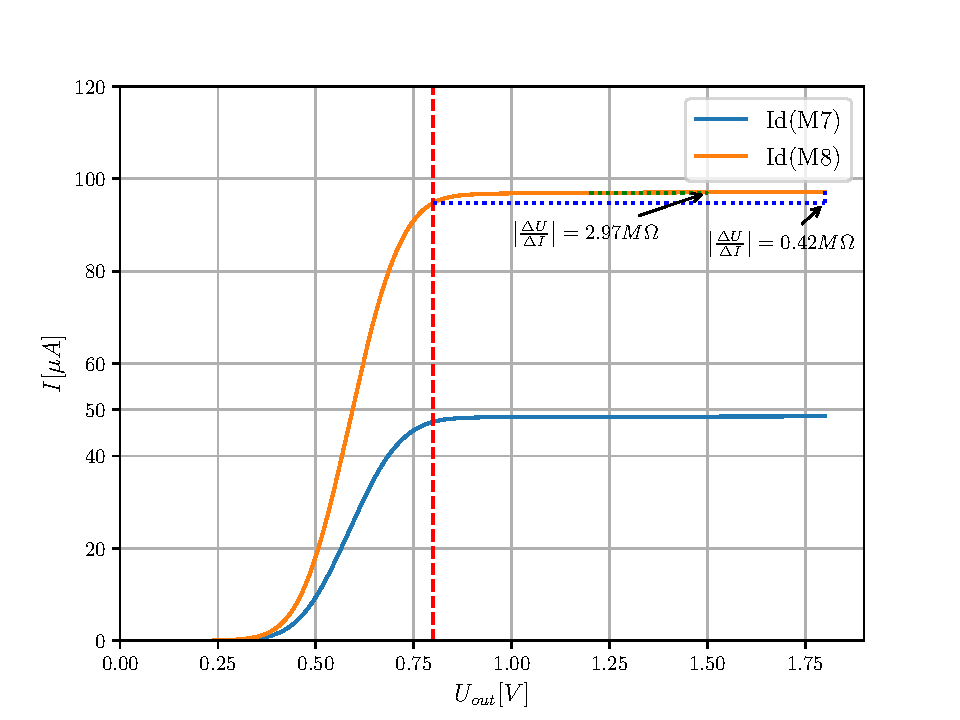
\includegraphics[width=0.8\textwidth]{2-3.pdf}
    \caption{DC analýza pro modifikované Wilsonovo proudové zrcadlo.}
    \label{fig:2-3-pdf}
\end{figure}